\documentclass{article}
\usepackage{ctex}
\usepackage{bm}
\usepackage{bbm}
\usepackage{amsmath}
\usepackage{amsthm}
\usepackage{algorithm,algorithmic}
\usepackage{url}
\usepackage{amssymb}
\usepackage{mathtools}
\usepackage{hyperref}
\newtheorem{theorem}{Theorem}
\newtheorem{example}{Example}
\newtheorem{lemma}{Lemma}
\def\E{\mathbb{E}}
\def\R{\mathbb{R}}
\DeclareMathOperator{\erf}{erf}
\title{A stochastic convex hull problem}
\begin{document}
\maketitle
\section{General statement}
$p_i$ are i.i.d. distributions in $d$ dimensional space
for $i=1,2,\dots, n, n+1$. We consider the event
$A_n =\{p_{n+1} \in ConvexHull\{p_1,
\dots, p_n\} \}$. $P(A_n)$ is also called
the probability content.
$P(A_n^c)$ increases if $d$ increases,
and it decreases if $d$ increases.

Notice that the event $A^c_n$ is different
from the event that $p_1, \dots, p_{n+1}$
are in convex position.

According to the survey article
\cite{barany2008random},
the problem originally comes from Sylvester's four point problem
in 1864. Then there are two directions afterwards.
One is studying the probability of all points are in convex
position, denoted as $p(n, K)$ in $d$ dimension where $K$ is the convex body
and $n$ is the number of points.
The other direction is to study $P(A_n)$.
The second direction diverges from the first direction
from the paper of Rényi in 1963 \cite{renyi1963konvexe}.

In the paper of Rényi, both the uniform distribution in a bounded region
and the normal distribution is considered.
The setting is constrained in a 2d plane.
When the points follow uniform distribution
in a unit circle, the asymptotic behavior
of the number of vertices is $cn^{1/3}$.
For the standard normal distribution in a plane,
$\E[V_n] \sim 2\sqrt{2\pi \log n}$.

Later on, in the paper of Hervé Raynaud (in the year 1970)
\cite{raynaud1970enveloppe},
the results
of Rényi are extended to higher dimensions.
Both Rényi and Raynaud
based their deductions on integration techniques.
Afterwards, discrete mathematics has been
employed to prove these old results (only the order
is recoverable) \cite{har2011expected}.
\section{Asymptotic result}
In this section, we review two important asymptotic result,
which is obtained in \cite{raynaud1970enveloppe}.
\begin{theorem}
    Let $X_1, \dots, X_n$ be i.i.d. random variables
    drawn from uniform distribution in a $d$-dimensional sphere.
    $H$ is the convex hull of $X_1, \dots, X_n$, which is also
    a random object.
    Then the expected number of vertices of $H$ is
    \begin{equation}
    \E[V_n] \sim f(d)n^{\frac{d-1}{d+1}}
    \end{equation}
    The asymptotic relationship holds when $n\to \infty$.
\end{theorem}
\begin{theorem}\label{thm:x1xnvn}
    Let $X_1, \dots, X_n$ be i.i.d. random variables
    drawn from standard normal distribution in a $d$-dimensional space.
    Then the expected number of vertices of $H$ is
    \begin{equation}
    \E[V_n] \sim g(d) (\log n)^{\frac{1}{2}(d-1)}
    \end{equation}
\end{theorem}
The above two theorems rely on the relationship between
$V_n$ and $F_n$(the $(d-1)$-dimensional faces of $H$).

\begin{equation}\label{eq:fv}
    F_n = (d-1) V_n - d^2 + d + 2
\end{equation}
Using mathematical induction to prove
\eqref{eq:fv}.

% Über die konvexe Hülle von n zufällig gewälhlten Punkten
Below we illustrate the techniques used to prove Theorem
\ref{thm:x1xnvn} by letting $d=2$.
That is, we will show that
\begin{equation}
    \E[V_n] \sim 2\sqrt{2\pi \log n}
\end{equation}
starting from
\begin{equation}
    \E[V_n] \sim \frac{n^2}{\sqrt{\pi}}
    \int_{0}^{+\infty} \Phi(p)^{n-2}e^{-p^2}dp
\end{equation}
The first observation is that we can use the approximation
$\Phi(p) = 1-\frac{\exp(-p^2/2)}{\sqrt{2\pi} p}$
when $p$ is large.
Given any $\epsilon>0$, the maximal value of $\Phi(p)^{n-2}e^{-p^2}$
is achieved within the interval $[\sqrt{2\log n} - \epsilon, \sqrt{2\log n}]$
for sufficiently large $n$. We can use $\exp(-p^2/2) \sim \frac{1}{n}$
to estimate the boundary.
Therefore:
\begin{equation*}
    \E[V_n] \sim \frac{n^2}{\sqrt{\pi}}
    \int_{\sqrt{2\log n} - \epsilon}^{\sqrt{2\log n}}
    e^{-n\left(\frac{\exp(-p^2/2)}{\sqrt{2\pi}p}\right)-p^2}dp
\end{equation*}
We first make the transformation $u=\sqrt{2\log n} - p$.
\begin{equation}\label{eq:middle}
    \E[V_n] \sim \frac{1}{\sqrt{\pi}}
    \int_{0}^{\epsilon}
    e^{-\left(\frac{\exp(-u^2/2+u\sqrt{2\log n})}{\sqrt{2\pi}(\sqrt{2\log n}-u)}\right)+(2\sqrt{2\log n}u-u^2)}du
\end{equation}
Since $\epsilon $ can be sufficiently small, some terms of $u$
without the coefficient $\sqrt{\log n}$ contribute minor to the integral.
And we can use $u=0$ as an approximation. Therefore,
\eqref{eq:middle} reduces to
\begin{equation*}
    \E[V_n] \sim \frac{1}{\sqrt{\pi}}
    \int_{0}^{\epsilon}
    e^{-\left(\frac{\exp(u\sqrt{2\log n})}{\sqrt{2\pi}(\sqrt{2\log n})}\right)+2\sqrt{2\log n}u}du
\end{equation*}
The next step is to let $t=\sqrt{2\log n} u$, then we have
\begin{equation*}
    \E[V_n] \sim \frac{1}{\sqrt{\pi} \sqrt{2\log n}}
    \int_{0}^{\epsilon \sqrt{2\log n}}
    e^{-\left(\frac{\exp(t)}{2\sqrt{\pi\log n}}\right)+2t}dt
\end{equation*}
Finally, we use $v=\frac{e^t}{2\sqrt{\pi \log n}}$,
then
\begin{equation*}
    \E[V_n] \sim \frac{(2\sqrt{\pi \log n})^2}{\sqrt{\pi} \sqrt{2\log n}}
    \int_{0}^{+\infty}
    e^{-v}vdv = 2\sqrt{2\pi \log n} \approx 5.01 \sqrt{\log n}
\end{equation*}
The above deduction can be extended to handle $d\geq 2$.
\section{Two dimensions}
$(x_i, y_i) \sim p(x,y)$ are i.i.d. distributions
for $i=1,2,\dots, n, n+1$. We consider the event
$A_n =\{(x_{n+1}, y_{n+1}) \in ConvexHull\{(x_1, y_1),
\dots, (x_n, y_n)\} \}$. We give a lower bound on $A_n^c$
(complement) as follows:
\begin{theorem}\label{thm:lower_bound}
    \begin{equation}
        P(A_n^c) \geq \frac{2}{n+1}
    \end{equation}
\end{theorem}
\begin{proof}
We use the method of projection to prove Theorem
\ref{thm:lower_bound}.
Consider a direction $(\cos\theta, \sin \theta)$
characterized by $\theta$. The projection of $(x_i, y_i)$
is given by $x_i \cos\theta + y_i \sin \theta$.
If $\exists \theta$ such that
$x_{n+1}\cos\theta + y_{n+1} \sin \theta$
is larger than $\max_{i=1,\dots, n} \{x_{i}\cos\theta +
y_{i} \sin \theta\}$ or smaller than
$\min_{i=1,\dots, n} \{x_{i}\cos\theta +
y_{i} \sin \theta\}$, $A_n^c$ happens.
Let $z_i = x_i \cos \theta + y_i \sin \theta$,
$z_{\max}=\max\{z_1, \dots, z_n\}$ and
$z_{\min}=\min\{z_1, \dots, z_n\}$.
Then we have $P(A_n^c) \geq P(\exists \theta, z_{n+1} > z_{\max})
+ P(\exists \theta, z_{n+1} < z_{\min})
\geq P(\theta=\theta', z_{n+1} > z_{\max})
+ P(\theta=\theta', z_{n+1} < z_{\min}) $.

Now we compute $P(z_{n+1} > z_{\max})$
for a number $\theta'$.
The PDF of $z=x\cos \theta' + y \sin \theta'$
is given as $p(z)=\int
\frac{p(x, \frac{z-x \cos \theta'}
{\sin \theta'})}{|\sin \theta'|}dx$.
$P(z_{n+1} > z_{\max}) = \int P(z_{\max} < z)p(z)dz
= \int F(z)^n p(z)dz$ where $F(z)$ is the CDF of the
random variable $Z$. Therefore, the integral evaluates
to $\frac{1}{n+1}$. Similarly,
$P(\theta=\theta', z_{n+1} < z_{\min})=
\frac{1}{n+1}$.
\end{proof}

If we consider two directions $\theta_1, \theta_2$
such that $z(\theta_1)=x\cos \theta_1 + y \theta_1$
is independent with $z(\theta_2)=x\cos \theta_2 + y \theta_2$.
For example, If $(X,Y)\sim \mathcal{N}(0, I_2)$,
we choose $\theta_1=0, \theta_2=\frac{\pi}{2}$.
Then
$
P(A_n^c) \geq
P(z_{n+1}(\theta_1)>z_{\max}(\theta_1)
\vee z_{n+1}(\theta_2)>z_{\max}(\theta_2)
\vee z_{n+1}(\theta_1)<z_{\min}(\theta_1)
\vee z_{n+1}(\theta_2)<z_{\min}(\theta_2)
)
$
Using the inclusion-exclusion principle,
we have
$
P(A_n^c) \geq
4P(z_{n+1}(\theta_1)>z_{\max}(\theta_1))
-4P(z_{n+1}(\theta_1)>z_{\max}(\theta_1)
\wedge z_{n+1}(\theta_1)<z_{\min}(\theta_1)
)
$.
Below we show that
\begin{equation}
    P(z_{n+1}(\theta_1)>z_{\max}(\theta_1)
\wedge z_{n+1}(\theta_1)<z_{\min}(\theta_1))
= \frac{1}{(n+1)^2}
\end{equation}
Let $z=z(\theta_1), z'=z(\theta_2)$,
then
\begin{align*}
    P(z_{n+1}(\theta_1)>z_{\max}(\theta_1)
    \wedge z_{n+1}(\theta_1)<z_{\min}(\theta_1))
    &= \iint P(z>z_1 \wedge z'>z'_1)^n p(z,z')dzdz'\\
    &= \iint F(z,z')^n p(z,z')dzdz'\\
    &= \iint F(z)^nF(z')^n p(z)p(z')dzdz'= \frac{1}{(n+1)^2}
\end{align*}
Therefore, $P(A_n^c) \geq \frac{4}{n+1} - \frac{4}{(n+1)^2}$.


Now we study the case for Gaussian.
Suppose $p(x,y)=\frac{1}{2\pi}\exp(-\frac{x^2}{2}
-\frac{y^2}{2})$,
then the exact formula for $P(A_n^c)$
is (See 1.7 of \cite{kabluchko2020absorption})
\begin{equation}\label{eq:gaussian_2d}
    P(A_n^c) = \frac{n}{\sqrt{\pi}} \int_{-\infty}^{+\infty}
    \Phi^{n-1}(u)e^{-u^2}du
\end{equation}
where $\Phi$ is the CDF of standard normal distribution.
We are interested in the decaying rate of $P(A_n^c)$
when $n\to \infty$, which is given in Lemma \ref{lem:gaussian}
\begin{lemma}\label{lem:gaussian}
If $(X,Y)\sim \mathcal{N}(0, I_2)$, then
\begin{align*}
P(A_n^c )\geq  \sqrt{2}\pi \left(\frac{2}{n+2}
-\frac{1}{n+1}
\right)
\end{align*}
\end{lemma}
\begin{proof}


First use integration by parts:
\begin{align*}
    P(A_n^c) &= \sqrt{2} \int_{-\infty}^{+\infty}
    e^{-u^2/2}d\Phi^n(u)
    =\sqrt{2} \int_{-\infty}^{+\infty}\Phi^n(u)
    ue^{-u^2/2}du \\
    &=2\sqrt{\pi} \int_{-\infty}^{+\infty}
    \Phi(u)^n ud\Phi(u)
\end{align*}
Then use change of variables ($y=\Phi^{n+1}(u)$):
\begin{align*}
    P(A_n^c) 
    =2\sqrt{\pi} \int_{0}^{1}z^n \Phi^{-1}(z)dz
\end{align*}
Using the relationship
$\Phi^{-1}(z)
= \sqrt{2} \erf^{-1}(2z-1)$
where $\erf$ is the error function,
we have
\begin{align*}
    P(A_n^c) 
    =\sqrt{2\pi} \int_{-1}^{1}
    \left(\frac{x+1}{2} \right)^n
    \erf^{-1} (x)dx
\end{align*}
Combining Lemma \ref{lem:bound_erf_integral},
we have $P(A_n^c) \geq  \frac{\sqrt{2}\pi}{n+1}$
approximately, which is a more tight lower bound than
Theorem \ref{thm:lower_bound}.
\end{proof}
\begin{lemma}\label{lem:bound_erf_integral}
    \begin{align}\label{eq:bound_erf_integral}
        \int_{-1}^{1}
    \left(\frac{x+1}{2} \right)^n
    \erf^{-1} (x)dx & \geq \sqrt{\pi}
    \left[\frac{2}{n+2} - \frac{1}{n+1}\right]
    \end{align}
\end{lemma}
\begin{proof}
    When $x>0$, we have the following inequality
    for the inverse error function $\erf^{-1}$
    (See the Maclaurin series of inverse error function
    \cite{inverseErf}).
    \begin{equation}\label{eq:ieq_erf_inverse}
        \erf^{-1}(x) \geq \frac{\sqrt{\pi}}{2}x
    \end{equation}
    In fact, we can replace
    $\erf^{-1}(x)$
    with $\frac{\sqrt{\pi}}{2}x$
    in \eqref{eq:bound_erf_integral} and obtain
    a lower bound.  This is based on the fact
    that $\erf$ is an odd function.
    The deduction is as follows:
    \begin{align*}  
        \int_{-1}^{1}
    \left(\frac{x+1}{2} \right)^n
    \erf^{-1} (x)dx
    &= \int_{-1}^{0}
    \left(\frac{x+1}{2} \right)^n
    \erf^{-1} (x)dx
    +\int_{0}^{1}
    \left(\frac{x+1}{2} \right)^n
    \erf^{-1} (x)dx \\
    &=-\int_{0}^{1}
    \left(\frac{1-x}{2} \right)^n
    \erf^{-1} (x)dx
    +\int_{0}^{1}
    \left(\frac{x+1}{2} \right)^n
    \erf^{-1} (x)dx \\
    &=    
    \int_{0}^{1}
    \left[\left(\frac{x+1}{2} \right)^n-
    \left(\frac{1-x}{2} \right)^n\right]
    \erf^{-1} (x)dx
    \end{align*}
    The term within the square bracket is larger
    than zero, therefore we can use
    the inequality \eqref{eq:ieq_erf_inverse}.

\end{proof}

\subsection{Special cases}
We consider $n=3 (d=2)$.
In this case, $P(A_n)$
is the expected volume of the triangles
whose three vertices are drawn randomly.

\begin{lemma}
    Under the Gaussian assumption of
    Lemma \ref{lem:gaussian},
    we have $P(A_n^c)=\frac{3}{2}
    (1-\frac{\arccos(1/3)}{\pi})
    \approx 0.91$.
\end{lemma}
\begin{proof}
From  \eqref{eq:gaussian_2d},
we should compute the integration
$\int_{\mathbb{R}} \Phi^2(x)e^{-x^2}
dx$.
From \cite{ruben1954moments},
this integral can be computed recursively
by the following formula:
\begin{align}
    \int_{\mathbb{R}} \Phi^n(x)e^{-x^2}
    dx &= \sqrt{\pi} \bar{V}_{n,n}(3) \\
    \bar{V}_{n,n}(x)
    &=\frac{1}{2^n}
    + \frac{n(n-1)}{4\pi}
    \int_{x}^{+\infty}
    \bar{V}_{n-2,n-2}(x'+2)
    \frac{dx'}{x'\sqrt{x'^2-1}}
    \label{eq:recursive}
\end{align}
Notice that \eqref{eq:recursive}
holds for $n\geq 2$. The starting
function is $\bar{V}_{0,0}(x)=1
,\bar{V}_{1,1}(x)=\frac{1}{2}$.
From \eqref{eq:recursive},
we have $\bar{V}_{n,n}(3)=
\frac{1}{4} + \frac{1}{2\pi}
(\frac{\pi}{2} - \arccos\frac{1}{3})
$
Then
\begin{equation}
\int_{\mathbb{R}} \Phi^2(x)e^{-x^2}
dx = \sqrt{\pi}(\frac{1}{2} - \frac{1}{2\pi}\arccos\frac{1}{3})
\end{equation}
Finally,
$P(A_3^c)=\frac{3}{\pi}
\int_{\mathbb{R}} \Phi^2(x)e^{-x^2}
=\frac{3}{2}
(1-\frac{\arccos(1/3)}{\pi})
$.
\end{proof}
If the points are drawn uniformly
from a square $[0,1]^2$, then
$P(A_3^c)=\frac{133}{144}$
(See the formula in \cite{valtr1995probability}
or the result on page 123 in \cite{henze1983random}).

When we require that the distribution is uniform in some bounded region.
An interesting conclusion (from the introduction of \cite{barany2008random})
is that $P(A_3)$ is the largest when
the distribution is uniform in a triangle and
smallest when the distribution is uniform in a disk.

\section{Expected number of vertices}
In section 3 of \cite{efron1965convex},
there is an elegant relationship between
$P(A_n^c)$ and the expected number of vertices
for a convex hull in 2d or 3d dimension.
\begin{equation}\label{eq:vertices}
P(A_n^c) = \frac{1}{n+1}\E[V_{n+1}]
\end{equation}
Using \eqref{eq:vertices}, 
\cite{efron1965convex} gives the formula
of $P(A_n^c)$ in 2d or 3d in Equation (7-5), (7-6).
$P(A_n)$ is also called the probability content.
However, the method used in 
\cite{efron1965convex} is hard to generalize in
higher dimensions.

Using the traditional conclusion on the
asymptotic analysis of $\E[V_n]$
in two-dimensional space,
we can obtain the following
asymptotic behavior for $P(A_n^c)$,
which is consistent with our lower bound
derived above, though the bound is
not tight in the sense of order.
\begin{theorem}
    $\E[V_n] = O(n^{1/3})$ for uniform distribution
    within a unit circle while
    $\E[V_n] = O(\log(n))$ for uniform distribution
    within a unit square.
\end{theorem}
A refinement for uniform distribution in a 2d circle states that $\E[V_n] \sim C n^{1/3}$ where
the constant $C$ is given as:
\begin{equation}\label{eq:Cn3}
    C = \Gamma\left(\frac{5}{3}\right) \left(\frac{16\pi^2}{3}
    \right)^{1/3} \approx 3.38
\end{equation}
This formula is derived in
Section 3 of \cite{renyi1963konvexe}.

Below we give another derivation of
\eqref{eq:Cn3} starting from (7.13)
of \cite{efron1965convex}, which states that
$\E[V_n] = \frac{2\pi^2}{3}\binom{N}{2}
\int_{-1}^{1} \Lambda_2^{N-2}(p)\lambda_2^3(p)dp$.

The first step is to shrink the integration interval.
\begin{align*}
    \int_{-1}^{1} \Lambda_2^{N-2}(p)\lambda_2^3(p)dp
    &=\int_{0}^{1} \left(\Lambda_2^{N-2}(p)
    +(1-\Lambda_2(p))^{N-2}\right)\lambda_2^3(p)dp
\end{align*}
Since $\Lambda_2(p) > \frac{1}{2}$ for $p>0$, the term
$(1-\Lambda_2(p))^{N-2}$ is neglectful when
$N$ is large.
Therefore, we only need to concern about
$\int_{0}^{1} \Lambda_2^{N-2}(p)\lambda_2^3(p)dp$,
Let $p=\cos\theta$, we then have
\begin{align*}
    \int_{0}^{1} \Lambda_2^{N-2}(p)\lambda_2^3(p)dp
    &=\frac{8}{\pi^3}\int_{0}^{\frac{\pi}{2}}
    \left(1+\frac{\sin\theta\cos\theta - \theta}{\pi}\right)^{N-2}
    \sin^4 \theta d\theta
\end{align*}
We can change the integral interval to $[0, \epsilon]$
for any constant $\epsilon<\frac{\pi}{2}$ without changing
the asymptotic behavior of the above value.
When $\epsilon$ is small, we can also use the approximation
$\theta \approx \sin\theta$. The term inside
the bracket becomes $1-\frac{1}{2}(2\theta)^3\frac{1}{6}\cdot \frac{1}{\pi}
=1-\frac{2\theta^3}{3\pi}$. We make the change
of variables from $\theta$ to $t$ by:
\begin{align*}
    \frac{t}{N} = \frac{2\theta^3}{3\pi}
\end{align*}
Then $\theta = \left(\frac{3\pi t}{2N}\right)^{1/3}$.
When $N$ is large, we have:
\begin{align*}
\int_{0}^{1} \Lambda_2^{N-2}(p)\lambda_2^3(p)dp
\sim \frac{8}{3\pi^3} \left(\frac{3\pi}{2N}\right)^{5/3}\int_0^{\infty}
\left(1-\frac{t}{N}\right)^{N-2}t^{2/3}dt
\sim\frac{8}{3\pi^3} \left(\frac{3\pi}{2N}\right)^{5/3}
\Gamma\left(\frac{5}{3}\right)
\end{align*}
Then the coefficient $C=\frac{\pi^2}{3}\cdot\frac{8}{3\pi^3} \left(\frac{3\pi}{2}\right)^{5/3}
\Gamma\left(\frac{5}{3}\right)$,
which reduces to \eqref{eq:Cn3}.
\subsection{Convex hull in 4d}
Euler's characteristic:
\begin{equation}
    V_N - E_N + F_N - \tilde{V}_N = 0
\end{equation}
\begin{itemize}
    \item $E_N$: the number of edges
    \item $F_N$: the number of faces (triangles)
    \item $\tilde{V}_N$: the number of volumes (tetrahedra)
\end{itemize}
\section{Bivariate Cauchy distribution}
Now we consider the case in 2d when the underlining
distribution is Cauchy (spherical symmetric). That is, the pdf is
\begin{equation}\label{eq:pxy_cauchy}
    p(x,y) = \frac{1}{2\pi} \frac{1}{(x^2+y^2+1)^{3/2}}
\end{equation}
The marginal distribution for $X$ is 1d Cauchy,
given by $p(x)=\frac{1}{\pi(1+x^2)}$, which
can be verified by direct integration of
\eqref{eq:pxy_cauchy}.

The 2d Cauchy specified in
\eqref{eq:pxy_cauchy} can be generated in the following way.
Let $y \sim U[0,1]$ and $\theta \sim
U[0, 2\pi]$. Then we obtain $r$
by $r=F^{-1}(y) = \frac{\sqrt{2y-y^2}}{1-y}$.
$F^{-1}$ is the inverse function
of $F(r)=1-(r^2+1)^{-1/2}$, the CDF of
$p(r)= \frac{r}{(r^2+1)^{3/2}}$.
Finally $x,y$ are obtained from polar transformation
of $(r,\theta)$.


According to (2.13) of \cite{efron1965convex},
the expected number of vertices is
\begin{equation}\label{eq:general_2d}
    \E(V_N) = 2\pi \binom{N}{2}
    \int_{\R}\E(|Y_2-Y_1| \Big\vert X_1= x, X_2=x)
    G^{N-2}_2(x) g^2_  2(x)dx
\end{equation}
we have $g_2(x) = p(x)$ and $G(x)=\frac{1}{2}+ \frac{1}{\pi}\arctan(x)$.
For the expectation term, we have the following lemma:
\begin{lemma}
    If $(X_1, Y_1), (X_2, Y_2)$ follow the bivariate Cauchy
    distribution, with pdf specified in \eqref{eq:pxy_cauchy}.
    Furthermore, these two random vectors are independent.
    Then we have,
    \begin{equation}
        \E(|Y_2-Y_1| \Big\vert X_1= x, X_2=x)
        = \frac{\pi}{2}\sqrt{1+x^2}
    \end{equation}
\end{lemma}
\begin{proof}
We list the definite and indefinite integrations
used in the proof first, which come from \cite{integration}.
\begin{align}
    \int_0^{\infty} \frac{dx}{(a^2+x^2)^2}
    & = \frac{\pi}{4a^3} \textrm{ See P108, 47. } \\
    \int \frac{dx}{(x^2+a^2)^{3/2}}
    & = \frac{x}{a^2\sqrt{x^2+a^2}}
    \textrm{ See P27 346.}\\
    \int \frac{x^2}{(c^2+x^2)^2}dx
    &=-\frac{x}{2(c^2+x^2)}
    +\frac{1}{2c}\arctan\frac{x}{c}
    \textrm{ See P12 137.}
\end{align}
We compute the integration directly:
\begin{align*}
    &\E\left(|Y_2-Y_1| \Big\vert X_1= x, X_2=x\right)
        =\frac{(1+x^2)^2}{4}\iint \frac{|y_1-y_2|}
        {(x^2+y_1^2+1)^{3/2}(x^2+y_2^2+1)^{3/2}}dy_1dy_2\\
        &=\frac{(1+x^2)^2}{2}\int_{\R}\frac{1}{(x^2+y_1^2+1)^{3/2}}
        dy_1\int_{y_1}^{+\infty}\frac{y_2-y_1}
        {(x^2+y_2^2+1)^{3/2}}dy_2 \\
        &=\frac{(1+x^2)^2}{2}\int_{\R}\frac{1}{(x^2+y_1^2+1)^{3/2}}
        \left(\frac{1}{\sqrt{1+x^2+y_1^2}}-y_1\left[\frac{1}{x^2+1}
        -\frac{y_1}{(1+x^2)\sqrt{1+x^2+y_1^2}}\right]\right)dy_1\\
        &=\frac{(1+x^2)^2}{2} \left(\frac{\pi}{2(1+x^2)^{3/2}}
        +\frac{\pi}{2(1+x^2)^{3/2}}\right)\\
        &=\frac{\pi}{2}\sqrt{1+x^2}
\end{align*}
\end{proof}
\begin{lemma}
    For bivariate Cauchy distribution,
$\lim_{N\to \infty}\E(V_N) = \frac{\pi^2}{2} \approx 4.93$.
\end{lemma}
\begin{proof}
From \eqref{eq:general_2d},
we have
\begin{equation*}
\E(V_N) = N(N-1)\pi \frac{\pi}{2}\int_{\R}
\sqrt{1+x^2}\frac{1}{\pi^2 (1+x^2)^2}(\frac{1}{2}
+\frac{1}{\pi}\arctan x)^{N-2}dx
\end{equation*}
Using the relationship $\arctan x =
\frac{\pi}{2} - \arctan \frac{1}{x}
$, we have (for any given $K>0$):
\begin{align*}
    \E(V_N) &\sim \frac{N^2}{2}\int_{K}^{+\infty}
    \frac{1}{(1+x^2)^{3/2}}
    \left(1-\frac{1}{\pi}\arctan \frac{1}{x} \right)^{N-2}dx\\
    &=\frac{N^2}{2}\int_{0}^{1/K}
    \frac{y}{(1+y^2)^{3/2}}
    \left(1-\frac{1}{\pi}\arctan y\right)^{N}dy\\
\end{align*}
When $y$ is small, $\arctan y \approx y$ (Taylor expansion).
Therefore, we can replace $\arctan y$ by $y$ without changing the
asymptotic behavior of the above expression.
Then making another change of variables by
$y=\frac{\pi}{N}t$:
\begin{align*}
    \E(V_N) &\sim \frac{\pi^2}{2}\int_{0}^{N/(K\pi)}
    \frac{tN^3}{(N^2+\pi^2 t^2)^{3/2}}
    \left(1-\frac{t}{N}\right)^{N}dt\\
    &\sim \frac{\pi^2}{2}\int_{0}^{+\infty}
    \frac{tN^3}{(N^2+\pi^2 t^2)^{3/2}}
    e^{-t}dt \sim  \frac{\pi^2}{2}
\end{align*}
\end{proof}
Empirical verification shown in Figure \ref{fig:2d_cauchy}. Use 1000 samples to compute $\E(V_N)$
for each $N$. Notice that as $N$ is large, the expected
number of vertices tend to be a constant (no more than 5).
This behavior is different with Gaussian or unit circle.

\begin{figure}[!ht]
    \centering
    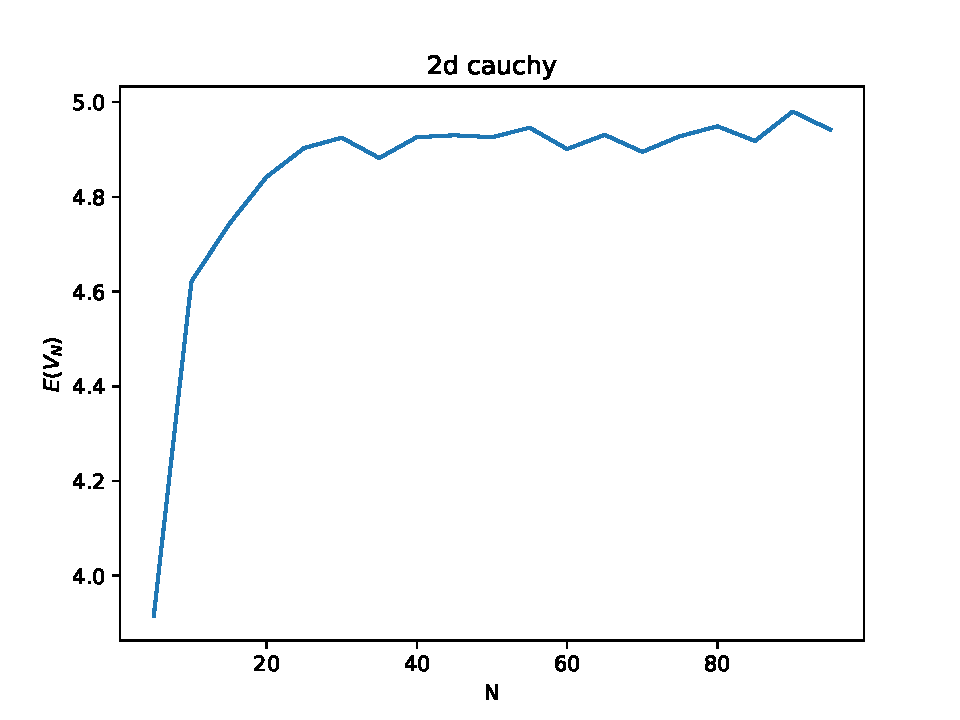
\includegraphics[width=0.6\textwidth]{2d_cauchy_vertices.pdf}
    \caption{}\label{fig:2d_cauchy}
\end{figure}

\section{A high dimensional ball}
Suppose $X$ is an n dimensional random gaussian vector
sampled from
$\mathcal{N}(\bm{0}, I_n)$. The upper bound of probability that it
falls within a hyperball with radius $R$ is computed
as follows:
\begin{align*}
    P(||X||\leq R) &= \int_{x_1^2 + \dots + x_n^2 \leq R^2}
    \frac{1}{(2\pi)^{n/2}}
    e^{-\frac{x_1^2 + \dots x_n^2}{2}}
    dx_1 \dots dx_n\\
    &= \frac{S_{n-1}(1) }{(2\pi)^{n/2}}
    \int_0^R r^{n-1} e^{-r^2/2}dr
    \\
    &=\frac{2\pi^{n/2}}{(2\pi)^{n/2}\Gamma(n/2)}
    \int_0^R r^{n-1} e^{-r^2/2}dr \\
    &=\frac{2\pi^{n/2}}{(2\pi)^{n/2}\Gamma(n/2)}
    \int_0^R r^{n-1} e^{-r^2/2}dr \\
    &=\frac{1}{\Gamma(n/2)}
    \int_0^{\frac{R^2}{2}} x^{\frac{n}{2} - 1} e^{-x}dx\\
    &=\frac{\gamma(n/2, \frac{R^2}{2})}{\Gamma(n/2)}
\end{align*}
We can use the recurrence relation for the
incomplete gamma function $\gamma(s,x)$:
\begin{equation}
    \gamma(s+1, x)
    = s\gamma(s, x) - x^s e^{-x}
\end{equation}
We consider the recurrence formula for the
following sequence:
$a_{n+1} = n a_n - bk^n$.
Dividing both sides by $n!$, we obtain
$\frac{a_{n+1}}{n!} =
\frac{a_n}{(n-1)!} - b\frac{k^n}{n!}$.
Therefore, $\frac{a_n}{(n-1)!} = a_1 - b\sum_{i=1}^{n-1}
\frac{k^i}{i!}$ while $a_1 = \gamma(1, k)=1-e^{-k}$
and $b=e^{-k}$.
$\frac{a_n}{(n-1)!} = e^{-k}(e-\sum_{i=0}^{n-1} \frac{k^i}{i!})
\sim e^{-k}\frac{k^n}{n!}$.
Therefore, suppose $n$ is an even number,
$P(||X||\leq R) \sim e^{-k}\frac{(R^2/2))^n}{n!}$.
The decaying rate is faster than exponential rate.

A looser bound is obtained by replacing the hyperball
with a bounding hypercube. Then
$P(||X||\leq R) \leq P(|X_1|\leq R)^n$, which is an
exponential rate.

\section{Crofton's formula}
This part mainly consults \cite{crofton}.

Crofton's formula gives a way to compute the arc length
by integration. Suppose we have a two dimensional
parametrized curve $\gamma: [0, 1] \to \mathbb{R}^2$.
Then the arc length of $\gamma$ is
\begin{equation}\label{eq:gamma}
    len(\gamma) = \frac{1}{2}\iint n(p, \theta)
    dp d\theta
\end{equation}
where $p, \theta$ is the polar coordinate representation
of a straight line. $n(p, \theta)$ is the number of times the 
straight line intersects the curve. The integration
in \eqref{eq:gamma} is over $p\in [0, +\infty)$
and $\theta \in [0, 2\pi]$.
\begin{example}
    The perimeter of the circle $x^2+y^2=r^2$.
    Using the integration formula \eqref{eq:gamma},
    we obtain $\frac{1}{2}\int_{0}^{2\pi} d\theta \int_0^r 2 dp=2\pi r$.
\end{example}
\begin{example}
    The line segment $0\leq x \leq 1, y=0$.
    The integral is $\frac{1}{2}\int_0^1 2 dp
    \int_0^{\arccos p} d\theta =
    \int_0^1 \arccos p dp=1$.
\end{example}
\bibliographystyle{plain}
\bibliography{ref.bib}
\end{document}



